\documentclass[12pt,a4paper,oneside]{book}
\usepackage[utf8]{inputenc}
\usepackage{amsmath}
\usepackage[spanish, es-tabla]{babel}
\usepackage{amsfonts}
\usepackage{amssymb}
\usepackage{multirow, array} 
\usepackage{chngcntr}
\usepackage{graphicx}
\usepackage{subfig}
\usepackage{cite}

\title{}
\begin{document}
\begin{center}
\thispagestyle{empty}
\fontsize{11pt}{11pt}\selectfont 

%%%%%%%%%%%%%%%%%%% PORTADA %%%%%%%%%%%%%%%%%%%%%%%%
PLAN DE TRABAJO DE GRADO 

\vspace{3cm}

\textbf { DISEÑO E IMPLEMENTACIÓN DE UNA ESTACIÓN METEOROLÓGICA CON ÉNFASIS EN LA MEDICIÓN DE CAMPO ELÉCTRICO PARA OBSERVATORIOS DE RAYOS CÓSMICOS.}


\vspace{3cm}

{ Autores}
\\
{ LEONARDO ANTONIO FLÓREZ VILLEGAS \\
PEDRO ANDRÉS SALGADO MEZA}

\vspace{2cm}
{ Director}
\\
{ JESÚS PEÑA RODRÍGUEZ}\\
\vspace{2cm}
{ Codirectores}\\
{ LUIS ALBERTO NÚÑEZ DE VILLAVICENCIO MARTÍNEZ} \\
{ JAIME GUILLERMO BARRERO PÉREZ } \\
\vspace{2cm}
{ ESCUELA DE INGENIERÍAS ELÉCTRICA, ELECTRÓNICA Y TELECOMUNICACIONES
}\\
{ UNIVERSIDAD INDUSTRIAL DE SANTANDER}\\
{ BUCARAMANGA}\\
{ 2019}

  \end{center}
\large

%%%%%%%%%%%%%%%%%%%%%%%%%%%%%%%		TABLA DE FIRMAS
\newpage
\begin{center}
\thispagestyle{empty}
\begin{table}[h!]
\centering
\begin{tabular}{|l|l|l|}
\hline
 ELABORADO POR:                                                         & REVISADO POR:                                                           & APROBADO POR:                                                                                                                                                                     \\ \hline
\begin{tabular}[c]{@{}l@{}} \\ \\ \\ \\ \rule{40mm}{0.2pt} \\ \scriptsize{Leonardo Antonio Flórez Villegas }\\ \tiny{\textit{Estudiante de Ingeniería Electrónica}}\\ \tiny{\textit{Código UIS:  2141838 }}\end{tabular} & \begin{tabular}[c]{@{}l@{}} \\ \\ \\ \\ \rule{40mm}{0.2pt} \\ \scriptsize{Ph.D.(c) Jesús Peña Rodríguez } \\ \tiny{\textit{Director del trabajo de grado}}\\ \\ \end{tabular}       & \begin{tabular}[c]{@{}l@{}}\scriptsize{Comité de trabajos de grado E\textsuperscript{3}T}\\ \scriptsize{Acta no. \rule{10mm}{0.2pt} del \rule{10mm}{0.2pt} de}\\ \scriptsize{\rule{20mm}{0.2pt} de 2019}\\ \scriptsize{código del trabajo:\rule{20mm}{0.2pt}}\\ \\ \\ \rule{40mm}{0.2pt}\\ \scriptsize{evaluador designado por el comite}\end{tabular} \\ \hline
\begin{tabular}[c]{@{}l@{}} \\ \\ \\ \rule{40mm}{0.2pt} \\ \scriptsize{Pedro Andrés Salgado Meza }\\ \tiny{\textit{Estudiante de Ingeniería Electrónica}}\\ \tiny{\textit{Código UIS: 2122966}}\end{tabular}      & \begin{tabular}[c]{@{}l@{}} \\ \\ \\ \\ \rule{40mm}{0.2pt} \\ \scriptsize{MSc. Jaime Guillermo }\\\scriptsize{Barrero Pérez}  \\ \tiny{\textit{Codirector del trabajo de grado}}\\ \\ \end{tabular} & \begin{tabular}[c]{@{}l@{}} \\ \\ \\ \\ \rule{40mm}{0.2pt}  \\ \scriptsize{Ph.D. Luis Alberto Núñez } \\\scriptsize{ de Villavicencio Martínez} \\ \tiny{\textit{Codirector del trabajo de grado}}\\ \\ \end{tabular}                                                                    \\ \hline
\end{tabular}
\end{table}
\end{center}

\noindent\makebox[\textwidth][c]{%
\begin{minipage}[b][8cm][c]{10cm}
\begin{center}
\textbf{Universidad Industrial de Santander (UIS)\\Documento Confidencial\\}
\end{center}
%\begin{center}
\scriptsize{Ni la totalidad ni parte de este documento puede reproducirse, almacenarse o transmitirse por algún procedimiento electrónico o mecánico, incluyendo fotocopias, grabación magnética o electrónica o cualquier medio de almacenamiento de información y sistemas de recuperación, sin permiso escrito de la UNIVERSIDAD INDUSTRIAL DE SANTANDER.\\Este es un documento interno de la UIS.  Al recibirlo no podrá pasarlo a persona alguna excepto las que se le indique en la lista de distribución autorizada por la UIS. Cualquier persona externa a la UIS que utilice la información en este documento asume la responsabilidad por su empleo.\\}
%\end{center}
\begin{center}
\textbf{© Universidad Industrial de Santander (UIS) – 2019}
\end{center}

\end{minipage}}
%%%%%%%%%%%%%%%%%%%%%%%%%%%%%%%%% GLOSARIO %%%%%%%%%%%%%%%%%%
%\newpage

%\chapter*{Glosario}


%\begin{description}
 %   \item[HV:] Alto voltaje (por sus siglas en inglés %High Voltage).
   
%\end{description}

\newpage
%%%%%%%%%% CONTENIDO %%%%%%%

\tableofcontents % indice de contenidos

\cleardoublepage
\addcontentsline{toc}{chapter}{Lista de figuras} % para que aparezca en el indice de contenidos
\listoffigures % indice de figuras

\cleardoublepage
\addcontentsline{toc}{chapter}{Lista de tablas} % para que aparezca en el indice de contenidos
\listoftables % indice de tablas



%%%%%%%%% FICHA DE RESUMEN %%%%%%%%%%%%%

\newpage
\markboth{FICHA RESUMEN}{}
\addcontentsline{toc}{chapter}{Ficha Resumen}

\thispagestyle{empty}
\begin{center}
\begin{Large}
\textbf{FICHA RESUMEN}
\end{Large}
\end{center}


\begin{table}[h!]
\centering
\begin{tabular}{p{3cm} p{15mm}}
\cline{2-2}
\multicolumn{1}{l|}{{\bf Título}}                                                                                         & \multicolumn{1}{l|}{\begin{tabular}[c]{@{}l@{}} Diseño e implementación de una estación meteorológica\\ con énfasis en la medición de campo eléctrico para\\ observatorios de rayos cósmicos. \end{tabular}}                                                                                                  \\[0.2cm] \cline{2-2} \noalign{\smallskip}

\cline{2-2}    

\multicolumn{1}{l|}{{\bf \begin{tabular}[c]{@{}l@{}}Autores:\end{tabular}}}          & \multicolumn{1}{l|}{\begin{tabular}[c]{@{}l@{}}
Leonardo Antonio Flórez Villegas\footnotemark,\\ leonardo.florez@correo.uis.edu.co \\
Pedro Andrés Salgado Meza\footnotemark,\\ pedro.salgado@saber.uis.edu.co
\end{tabular}}   \\[0.4cm] \cline{2-2} \noalign{\smallskip}                                                                                                                         
\cline{2-2}    

\multicolumn{1}{l|}{{\bf \begin{tabular}[c]{@{}l@{}}Director:\end{tabular}}}          & \multicolumn{1}{l|}{\begin{tabular}[c]{@{}l@{}}
Jesús Peña Rodríguez\footnotemark,\\ jesus.pena@correo.uis.edu.co 
\end{tabular}}   \\[0.2cm] \cline{2-2} \noalign{\smallskip}                                                                         
\cline{2-2}    
\multicolumn{1}{l|}{{\bf \begin{tabular}[c]{@{}l@{}}Codirector:\end{tabular}}}          & \multicolumn{1}{l|}{\begin{tabular}[c]{@{}l@{}}
Luis Alberto Núñez de Villavicencio Martínez\footnotemark, \\lnunez@uis.edu.co \\ 
 Jaime Guillermo Barrero Pérez\footnotemark, \\jbarrero@uis.edu.co
\end{tabular}}   \\[0.2cm] \cline{2-2} \noalign{\smallskip}                                                                   
\cline{2-2}
\multicolumn{1}{l|}{{\bf \begin{tabular}[c]{@{}l@{}}Modalidad:\end{tabular}}}          & \multicolumn{1}{l|}{\begin{tabular}[c]{@{}l@{}}
Trabajo de investigación
\end{tabular}}   \\[0.2cm] \cline{2-2} \noalign{\smallskip}                                                                                                                         
\cline{2-2}
\multicolumn{1}{l|}{{\bf \begin{tabular}[c]{@{}l@{}}Duración:\end{tabular}}}          & \multicolumn{1}{l|}{\begin{tabular}[c]{@{}l@{}}
8 meses
\end{tabular}}   \\[0.2cm] \cline{2-2} \noalign{\smallskip}                                                                                                                         
\cline{2-2}
\multicolumn{1}{l|}{{\bf \begin{tabular}[c]{@{}l@{}}Entidades\\ Interesadas:\end{tabular}}}          & \multicolumn{1}{l|}{\begin{tabular}[c]{@{}l@{}}
- Universidad Industrial de Santander (UIS).\\
- Escuela de Ingenierías Eléctrica, Electrónica y Telecomunicaciones\\ \hspace{0.3cm}(E3T).\\
- Grupo de Investigación en Relatividad y Gravitación, (GIRG).\end{tabular}}   \\[0.4cm] \cline{2-2} \noalign{\smallskip}


\cline{2-2}
\multicolumn{1}{l|}{{\bf \begin{tabular}[c]{@{}l@{}}Objetivo\\ General:\end{tabular}}}          & \multicolumn{1}{l|}{\begin{tabular}[c]{@{}l@{}}
Diseñar un prototipo de estación meteorológica autónoma\\ de bajo costo, enfocada a la medición de variables atmosféricas\\ de tormentas eléctricas.\end{tabular}}   \\[0.4cm] \cline{2-2} \noalign{\smallskip}


\end{tabular}
\end{table}

\footnotetext[1]{Estudiante de Ingeniería Electrónica de la UIS. Código: 2141838.}
\footnotetext[2]{Estudiante de Ingeniería Electrónica de la UIS. Código: 2122966.} 
\footnotetext[3]{ Ph.D(c) en Física.}
\footnotetext[4]{Profesor Titular UIS.} 

\chapter{Descripción del trabajo}

En la ejecución de este proyecto se fabricará un prototipo de estación meteorológica, que permita la medición del campo eléctrico atmosférico rápido (0.1 MHz – 1 MHz) y lento (0.1 Hz – 1 kHz) con el fin de estudiar posibles correlaciones entre sus variaciones y el aumento o disminución de flujo de CRs (Rayos Cósmicos) a nivel de suelo.\\\\
%%%%%%%%
%Con los datos registrados y apoyados en las mediciones realizadas por prototipos distribuidos estratégicamente en una red de estaciones%
%%%%%%%%
El prototipo integrará además la medición de otras variables meteorológicas como la temperatura, presión atmosférica y humedad así como un GPS para establecer la ocurrencia temporal de los eventos registrados. El trabajo a realizar se divide en 4 fases:  
%debe cumplir con lineamientos de diseño respecto al tamaño, precio y consumo energético. Por tal razón, se debe establecer cuales variables son relevantes, el costo del hardware que permita medirlas y el tamaño de diseño. El trabajo a realizar se dividió en 4 fases:
\begin{itemize}
    \item Estado del arte y documentación.
    \item Diseño de sensores de campo eléctrico.
    \item Diseño y construcción del prototipo.
    \item Pruebas y análisis de datos. 
\end{itemize}




\large 

\newpage

%%%%%%%%%%%%%%%%%%%%% PLANTEAMIENTO DEL PROBLEMA  %%%%%%%%%%%%%%%%%%%%%%%%%%https://www.overleaf.com/project/5cc1c08ea595920ee3c78bc9
\newpage 
\chapter{Planteamiento del Problema}
Los rayos cósmicos son partículas altamente energéticas que llegan a nuestro planeta tras propagarse por el espacio. Proceden de fenómenos astrofísicos violentos tales como fulguraciones solares o explosiones de supernovas. Cuando un rayo cósmico ingresa a la atmósfera, interactúa con los átomos que la componen creando chubascos de partículas secundarias, también llamados lluvias aéreas extendidas (EAS).\\\\
Los rayos cósmicos secundarios pueden ser usados en diferentes aplicaciones, que abarcan desde el entendimiento de la naturaleza de los rayos cósmicos primarios, hasta aplicaciones en clima espacial, física de altas energías \cite{Spurio2015}, muongrafía \cite{kaiser2018muography} entre otras.\\\\
Debido a que la mayoría de partículas generadas en la atmósfera poseen carga, estas pueden ser afectadas por los campos eléctricos presentes durante las tormentas, causando un aumento en el flujo de secundarios a nivel del suelo. Actualmente se han realizado algunos estudios correlacionando ambos fenómenos. Wang et al. \cite{wang2012effect} y Alexeenko et al. \cite{alexeenko2002transient} concluyeron que el número de muones detectados a nivel de suelo es modulado por la magnitud del campo eléctrico atmosférico. Bartoli et al. \cite{bartoli2018observation} observaron un decrecimiento en el número de electrones registrados por ARGO-YBJ durante tormentas eléctricas, mientras que Huang et al. \cite{zhao2019effects} encontraron que la variación en el número de electrones y gammas depende de la polaridad del campo eléctrico atmosférico.\\\\
%Por otra parte, las discusiones a cerca de la aceleración causada por el campo eléctrico atmosférico, sobre partículas secundarias cargadas han prevalecido en la literatura científica por mucho tiempo. Algunos estudios han correlacionado el cambio en el flujo de secundarios detectados a nivel de suelo con el campo eléctrico durante tormentas eléctricas. Wang et al. \cite{wang2012effect} y Alexeenko et al. \cite{alexeenko2002transient} concluyeron que el número de muones detectados a nivel de suelo es modulado por la magnitud del campo eléctrico atmosférico. Bartoli et al. \cite{bartoli2018observation} observaron un decrecimiento en el número de electrones registrados por ARGO-YBJ durante tormentas eléctricas, mientras que Huang et al. \cite{zhao2019effects} encontraron que la variación en el número de electrones y gammas depende de la polaridad del campo eléctrico atmosférico.\\\\
%%
Sin embargo, el estudio de eventos transitorios en el flujo de CRs secundarios se ha limitado en profundidad ya que el registro de datos de campo eléctrico atmosférico durante tormentas es escaso en los observatorios de CRs. Por esta razón, es necesario conocer la intensidad y las variaciones del campo eléctrico atmosférico con el fin de correlacionar su efecto sobre los transitorios en la tasa de partículas detectadas a nivel de suelo.

%el registro de datos de campo eléctrico atmosférico durante tormentas eléctricas es escaso en los observatorios de CRs, por lo que el estudio de eventos transitorios en el flujo de CRs secundarios se ha limitado en profundidad. Por esta razón es necesario conocer la intensidad y las variaciones del campo eléctrico atmosférico con el fin de correlacionar su efecto sobre los transitorios en la tasa de partículas detectadas a nivel de suelo.
%%

 
%%%%%%%%%%%%%%%%%%%%% JUSTIFICACIÓN  %%%%%%%%%%%%%%%%%%%%%%%%%%https://www.overleaf.com/project/5cc1c08ea595920ee3c78bc9
\newpage 
\chapter{Justificación}
%Los CRs son partículas que llegan desde el espacio y bombardean constantemente a la Tierra desde todas las direcciones \cite{cronin1999cosmic}. Cuando un rayo cósmico penetra la atmósfera, colisiona con átomos y moléculas en la atmósfera creando partículas secundarias. Algunas de ellas pueden alcanzar el suelo, donde pueden ser medidas, infiriendo de esta forma las propiedades de los rayos primarios que las generaron \cite{muraki2004effects}.\\
El campo eléctrico atmosférico varia desde $\pm$ 100 V/m en condiciones ambientales normales, hasta $\pm$ 100 kV/m durante tormentas. Los CRs secundarios cargados, principalmente electrones y positrones, pueden ser acelerados bajo la influencia de dicho campo \cite{macgorman1998electrical,marshall2005observed}, generando un efecto de RREA (por sus siglas en inglés Relativistic Runaway Electron Avalanches) \cite{dwyer2011low} que aumentan el conteo de eventos en los detectores a nivel de suelo.\\\\
En campos eléctricos negativos (es decir, aceleración de partículas con carga negativa hacia abajo), las tasas de conteo de partículas secundarias a nivel de suelo aumentan con la intensidad del campo eléctrico. En campos eléctricos positivos, las tasas disminuyen con la intensidad del campo \cite{dorman2013cosmic}. Estos resultados, por primera vez, dan una explicación coherente del origen de la variación del flujo de electrones o positrones observado durante décadas por los detectores de CRs a gran altitud durante las tormentas eléctricas \cite{Marteau-etal2012}.\\\\
Teniendo en cuentas los hechos anteriormente mencionados, un sistema de monitoreo de campo eléctrico, permitiría correlacionar la variación del campo eléctrico y la cantidad de partículas secundarias medidas por los detectores, y de esta manera entender los mecanismos atmosféricos de aceleración. 

\chapter{Objetivos}
\section{\textbf{Objetivo General}}

Diseñar un prototipo de estación meteorológica autónoma para la medición del campo eléctrico atmosférico en observatorios de astropartículas.


\section{\textbf{Objetivos Específicos}}

\begin{itemize}
    \item Consultar el estado del arte del estudio de tormentas eléctricas mediante estaciones meteorológicas.
    \item Diseñar e implementar un sensor de campo eléctrico rápido (0.1 MHz $–$ 1 MHz) y lento (0.1 Hz $–$ 1 kHz) para tormentas eléctricas.
    \item Implementar en la estación de monitoreo sensores complementarios de temperatura, presión, humedad y lluvia.
    \item Implementar mediante GPS la sincronización temporal de los eventos registrados.
    \item Desarrollar una interfaz gráfica para la visualización de los datos recolectados.
\end{itemize}

%%%%%%%%%%%%%%%%%%%%% Marco Teórico %%%%%%%%%%%%%%%%%%%%%%
\newpage
\chapter{Marco Teórico}

\section{Rayos cósmicos}

Los rayos cósmicos fueron descubiertos por el físico austríaco Víctor Hess en 1911. El experimento consistió en medir la radiación ionizante en la atmósfera usando en un globo aerostático. Hess esperaba observar una disminución en dicha radiación a medida que se alejaba de la superficie, sin embargo encontró un aumento, concluyendo que dicha radiación debía provenir de algún lugar fuera del planeta.\medskip

Los rayos cósmicos primarios pueden ser partículas subatómicas que viajan a grandes velocidades a través del espacio hasta llegar a nuestro planeta. Estas partículas son aceleradas por campos magnéticos presentes en los cuerpos astrofísicos ( estrellas, galaxias entre otras ) hasta que algunas culminan su trayectoria en la tierra. \medskip

%Las partículas con energías mayores a los $ 10^{15} eV $ son de origen extra-galáctico, puesto que para portar dichas energías han debido ser aceleradas distancias mucho mayores al ancho de la vía láctea.\medskip

Las partículas primarias interactúan con núcleos atómicos de los gases de la atmósfera terrestre produciendo una lluvia o cascada de partículas secundarias (EAS) las cuales pueden ser detectadas en la superficie de la tierra.\medskip



\begin{figure}[ht]
  \centering
  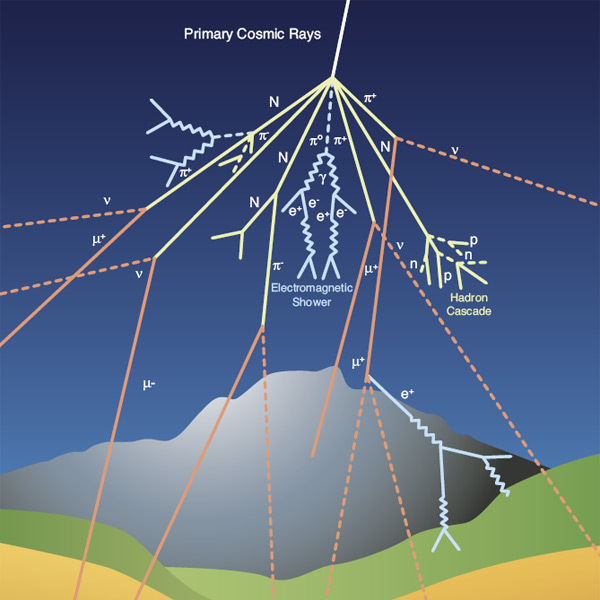
\includegraphics[width=0.6\textwidth]{c.jpg}
  \caption{Cascada de rayos cósmicos. Tomado de Página oficial del CERN}
  \label{fig1}
\end{figure}


La detección indirecta de rayos cósmicos se hace mediante observatorios basados en detectores Cherenkov de agua (WCD), centelladores, telescopios de fluorecensia, IACT (Telescopios de Cherenkov en el Aire) y antenas. Con los datos recolectados se reconstruyen la cascada de partículas secundarias para poder determinar dos cosas principalmente, qué partícula originó la cascada y cuál fue su dirección de incidencia. \medskip


\section{Influencia del campo eléctrico en CRs atmosféricos }

%Cuando los rayos cósmicos primarios entran en nuestra atmósfera y desencadenan las cascada de partículas secundarias se producen partículas como muones, electrones, positrones, fotones y hadrones. De estas,  3 primeras partículas tienen carga y por lo tanto se ven afectadas por campos eléctricos y magnéticos.\medskip

Las partículas secundarias se dividen en tres componentes: la electromagnética (electrones, positrones y fotones), la hadrónica y la penetrante (muones y neutrinos). En presencia de campos eléctricos mayores a 25 kV/m el número de partículas de la componente electromagnética aumenta \cite{colalillo2019}. 


%Cuando ocurre un evento de estos con condiciones climáticas normales, el campo eléctrico atmosférico es constante ( 100 V/m ) , pero durante una tormenta eléctrica, el campo eléctrico puede llegar hasta 20 kV/m presentando variaciones transitorias en intensidad y polarización.\medskip

Al exponer positrones y electrones a un campo eléctrico se observa una aceleración o desaceleración en ambas partículas dependiendo su polaridad, generando avalanchas subsecuentes \cite{zhao2019effects}.\medskip


\begin{figure}[ht]
  \centering
  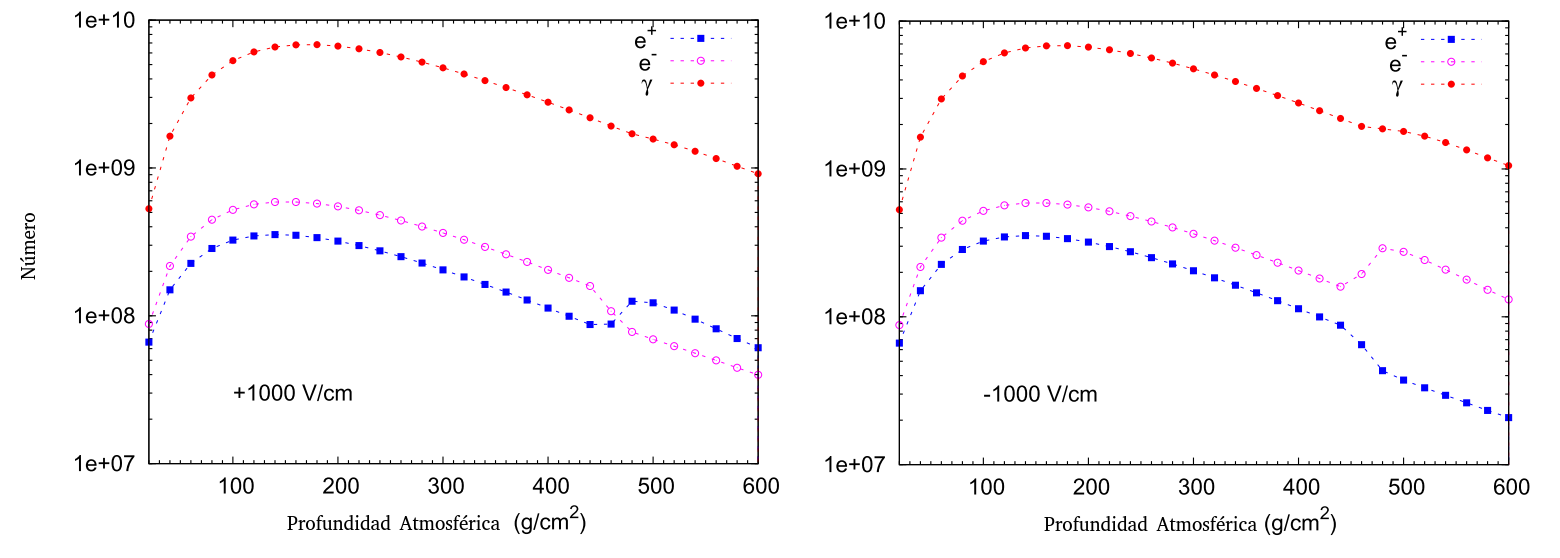
\includegraphics[width=1\textwidth]{All.png}
  \caption{Número de $e^{+}$ (azul), $e^{-}$ (rosado) y $\gamma$ (rojo) como función de la profundidad atmosférica con un campo eléctrico de 1 kV/m (izquierda) y -1 kV/m (derecha). Tomado de \cite{zhao2019effects} }
  \label{fig22}
\end{figure}

Como se puede apreciar en la Fig. \ref{fig22}, un campo eléctrico con polaridad negativa, donde las nubes tiene carga negativa y el suelo positiva, produce una aceleración en los electrones y un frenado en los positrones, además de un aumento en los fotones debido al Bremsstranhlung. Al invertir la polaridad del campo, los positrones son acelerados y los electrones desacelerados. \medskip

Este aumento en las partículas secundarias producidas durante las alteraciones del campo eléctrico en condiciones atmosféricas adversas puede atribuirse erróneamente a la energía de la partícula primaria que desencadenó la cascada. Por ello es importante lograr correlacionar este aumento en algunas partículas secundarias durante una tormenta con el campo eléctrico atmosférico.

\section{Campo eléctrico rápido y lento}

El planeta tierra contiene en su atmósfera gran cantidad de gases que son ionizados por los rayos cósmicos aumentando la conductividad del aire. La atmósfera terrestre es análoga a un gran condensador cuyo potencial puede llegar hasta los 300 kV \cite{ogawa1973analyses}.

En condiciones ambientales normales el campo eléctrico terrestre es constante, pero durante una tormenta este varia de forma escalonada, produciendo cambios que pueden durar desde 1 ms hasta 10 s, a este comportamiento se le conoce como campo eléctrico lento. Durante estos aumentos o disminuciones se producen transitorios, cuya frecuencia puede variar de 1 kHz a 1 MHz, los cuales son llamamos campo eléctrico rápido. \medskip

Para el monitoreo de éstos eventos se usan dos tipos de sensores, uno para el campo eléctrico rápido y otro para el campo eléctrico lento. \medskip

\subsection{Sensor de campo eléctrico lento tipo molino}

Este sensor consiste en un motor DC que lleva acoplado a su rotor un placa metálica (obturador giratorio) que obstruye la influencia del campo eléctrico atmosférico sobre el electrodo sensor como se puede ver en la Fig. \ref{figm}.

\begin{figure}[ht]
  \centering
  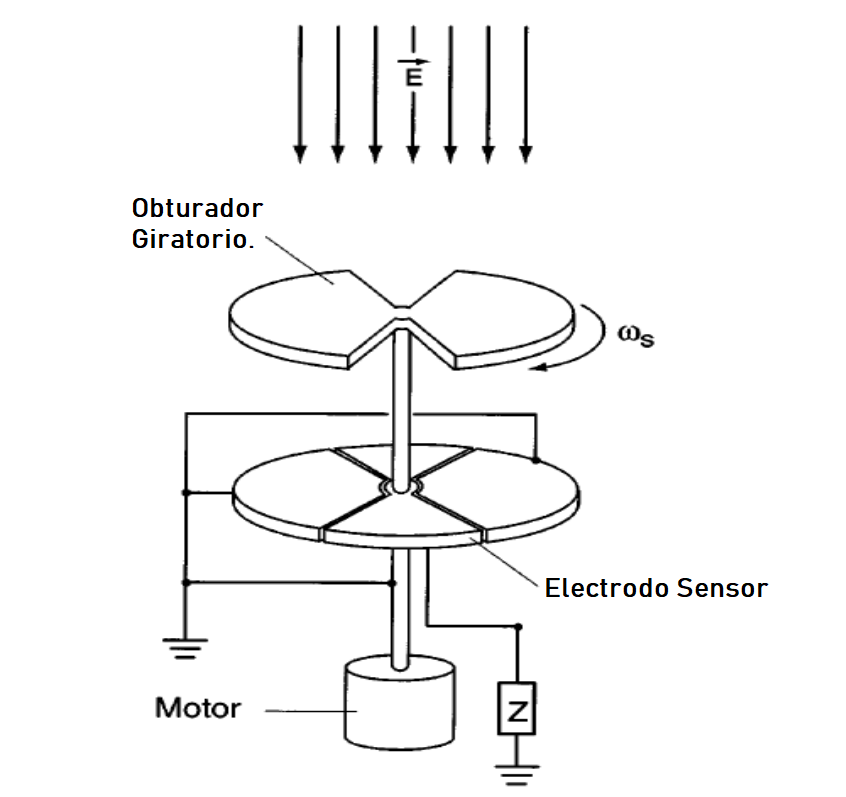
\includegraphics[width=0.55\textwidth]{Field_Mill.png}
  \caption{ Esquema básico del sensor de campo eléctrico tipo molino. La lámina obturadora controla de manera periódica la carga y descarga del plato sensible debido al campo eléctrico incidente. Tomado de \cite{ibrahim2011measurement} }
  \label{figm}
\end{figure}

La placa superior deja al descubierto gradualmente la lámina sensible permitiendo que esta se cargue debido al campo eléctrico atmosférico incidente. Luego la lámina sensible es cubierta por el obturador generando de esta manera su descarga. Como resultado se obtiene es una señal sinusoidal cuya frecuencia depende de la frecuencia de giro del motor y cuya amplitud es proporcional a al magnitud del campo eléctrico atmosférico \cite{mosquera2015}. 

La fase de la señal depende de la polarización del campo eléctrico y se determina mediante un \textit{encoder} que sensa el paso del obturador sobre la lámina sensible.

\subsection{Antena de platos paralelos}

Para lograr medir las variaciones de campo eléctrico rápido generalmente se utiliza una antena de placas paralelas como se muestra en la Fig. \ref{figc} \cite{ogawa1973analyses}. 

\begin{figure}[h!]
  \centering
  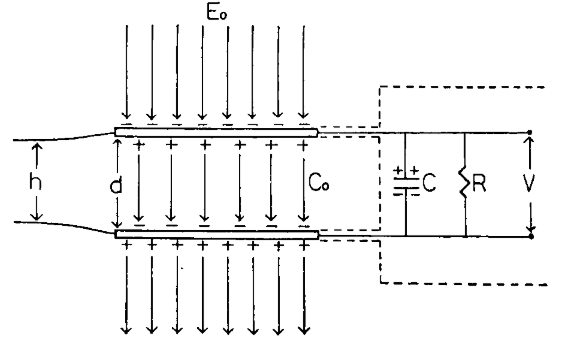
\includegraphics[width=0.7\textwidth]{Cap.png}
  \caption{ Sensor de placas paralelas. Tomado de  \cite{ogawa1973analyses} }
  \label{figc}
\end{figure}

Durante una tormenta eléctrica se presentan variaciones rápidas del campo que inducen cambios en la carga (corriente) en el plato sensible de la antena. La corriente generada es proporcional a la derivada del campo eléctrico,

\begin{equation}
    I = \frac{dQ}{dt} = A\epsilon_0 \frac{dE}{dt} 
\end{equation}

donde, $A$ es el área de la placa sensible y $\epsilon_0$ la permitividad del vacío.

Teniendo en cuenta lo anterior, a la salida de la antena se implementa un circuito integrador compuesto por un condensador $C$ y una resistencia $R$ que genera una señal de voltaje $V$ proporcional a la magnitud del campo eléctrico teniendo en cuenta la relación,

\begin{equation}
    V = \frac{1}{RC} \int I dt = \frac{\epsilon_0 A E}{C}
\end{equation}

%Esta carga genera una diferencia de potencial que es directamente proporcional al campo eléctrico atmosférico según la ecuación,\medskip
%Esta etapa se comporta como filtro pasa bajas, cuya frecuencia de corte debe ser lo suficiente grande, mayor a 1 MHz, por esta razón la capacitancia predominante debe ser la de la antena y el capacitor C debe tener una capacitancia mucho menor a esta. \medskip



%%%%%%%%%%%%%%%%%%%%% ALCANCES  %%%%%%%%%%%%%%%%%%%%%%%%%%
\newpage
%\chapter{Alcances}
 
%El proyecto plantea diseñar un prototipo de estación meteorológica autónoma de bajo costo para la medición de campo eléctrico atmosférico, con aplicación particular al estudio de CRs en observatorios de astropartículas.\\\\
%Durante su desarrollo, se investigarán los sensores que permiten medir las variables electro-atmosféricas, teniendo en cuenta la exactitud, precisión y costo del dispositivo.\\\\
%Se desea crear una nueva metodología para el diseño de sensores de campo eléctrico de bajo costo, además se apunta a la apropiación social del conocimiento local, haciendo posibles estudios en otras áreas del conocimiento donde se necesiten los datos adquiridos por la estación.\\\\ 
%La importancia de esta implementación se asegura por su aplicación directa al estudio de fenómenos de aceleración de rayos cósmicos en la atmósfera terrestre. De esta forma es posible diseñar una red de dispositivos conformando una red de monitoreo para la medición de las variaciones de campo eléctrico atmosférico y su relación con el conteo de CRs mediante detectores de astropartículas secundarias. 

%%%%%%%%%%%%%%%%%%%%%  Metodología%%%%%%%%%%
\newpage 

\chapter{Metodología}

\section{\textbf{Revisión bibliográfica}}
El punto de inicio de la investigación se establece con una revisión bibliográfica, sobre trabajos existentes en el área, esto nos va a permitir afrontar el problema desde diferentes perspectivas. 
\section{\textbf{Documentación del proyecto}}
En esta etapa se definen los métodos de medición del campo eléctrico en el desarrollo de una tormenta eléctrica. 
\section{\textbf{Selección de hardware}}
Después de haber establecido que variables tienen mayor relevancia en una tormenta eléctrica, se debe escoger un método de medición, y de transmisión de datos, seleccionando el hardware necesario para el funcionamiento de la estación siguiendo los lineamientos de tamaño, costo y consumo de energía.

\section{\textbf{Diseño de la arquitectura}}
Luego de haber seleccionado el hardware, se construye una arquitectura que integre el hardware y una topología de transmisión eficiente de datos. 
\section{\textbf{Construcción del prototipo}}
En esta etapa del proyecto se construirá el prototipo siguiendo una metodología escalonada, esto significa que se irá construyendo poco a poco de tal forma que se pueda realizar pruebas de cada parte de la estación por separado, luego se procederá a integrar el prototipo para las pruebas de funcionamiento conjunto. 

% Escuela de Física\\
% Universidad Industrial de Santander\\
% Correo:halley@uis.edu.co\\
% Teléfono:(+57-7)634 40 00 ext. 2741\\
% %Carrera 27 calle 9 ciudad universitaria\\
% %Edificio Ciencias Humanas, Oficina 504\\
% Bucaramanga,Colombia


\section{\textbf{Sistema de adquisición y transmisión
}}
Uno de los objetivos del proyecto es la transmisión de los datos atmosféricos a un aplicativo, por lo que se procederá a implementar dicha característica mediante alguna tecnología de transmisión eficiente.


\section{\textbf{Prueba de funcionamiento y validación
}}
Validar el funcionamiento de la estación juega un papel relevante en el presente proyecto, ya que garantizará que el producto soporta las condiciones ambientales a las que este expuesto durante el proceso de adquisición, la calidad y credibilidad de los datos. 

\section{\textbf{Informe final
}}
En este punto se va a realizar la integración de toda la información recolectada en cada fase y las conclusiones importantes en el informe final. 

 
%%%%%%%%%%%%%%%%%%%%% CRONOGRAMA DE ACTIVIDADES%%%%%%%%%%
\newpage 

\chapter{Cronograma de actividades}
Para llevar a cabo los objetivos del proyecto, se hace un planteamiento de las actividades a realizar en el transcurso de los 8 meses que se definió como duración del proyecto de grado.

\begin{figure}[ht]
  \centering
  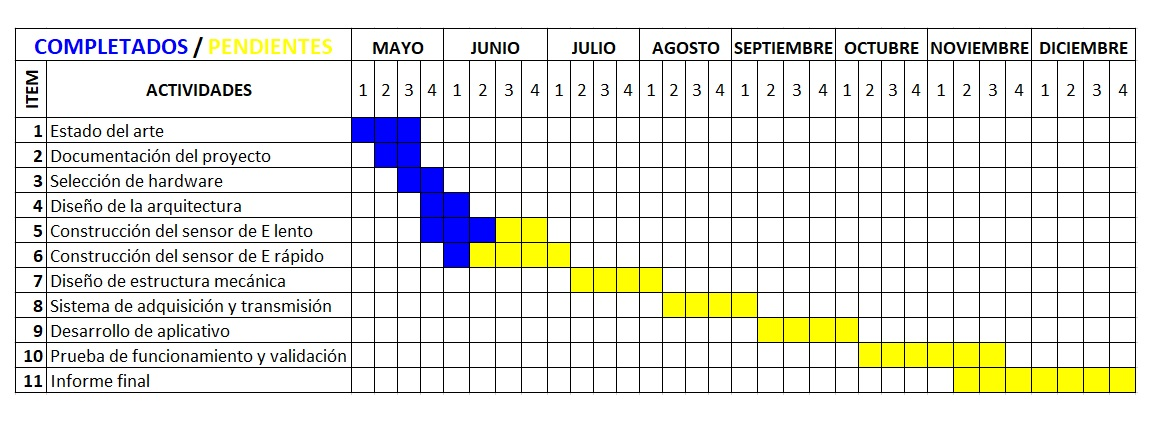
\includegraphics[width=\columnwidth]{CRONOGRAMA.jpg}
  \caption{Cronograma de actividades.}
\end{figure}



%%%%%%%%%%%%%%%%%%%%% RECURSOS E INFRAESTRUCTURA %%%%%%%%%%%%%%%%%%%%%%
\newpage 
\chapter{Recursos e Infraestructura}
\section{\textbf{Recursos Humanos}}

\begin{table}[htbp]
\begin{center}
\begin{tabular}{|p{2cm}|p{7cm}|}\hline
\hline
Función & Descripción \\
\hline    \hline
Director  & Decide sobre los recursos, determina y asigna las tareas. \\ \hline
Codirectores  & Deciden sobre los recursos, riesgos del proyecto y asignan tareas.  \\ \hline
Autores  & Estudiantes de Ingeniería Electrónica encargados de investigar, documentar y desarrollar el proyecto de grado.  \\ \hline
\end{tabular}
\caption{Recursos Humanos.}
\label{Tabla: Recursos Humanos}
\end{center}
\end{table}
 
\section{\textbf{Materiales}}
La siguiente lista de materiales se va a solicitar a la universidad por medio del grupo de investigación GIRG y se encontrarán disponibles en el laboratorio del grupo Halley para su uso.\\\\

\begin{table}[htbp]
\begin{center}
\begin{tabular}{|p{2cm}|p{7cm}|}\hline
\hline
Cantidad & Descripción\\
\hline  \hline
3 & Sensor de presión atmosférica LPS35HW\\ \hline
3 & Sensor de campo eléctrico \\ \hline
3 & Sensor de temperatura MCP9808 \\ \hline
3 & Sensor de lluvia RG11 \\ \hline
3 & Sensor de rayos AS3935 \\ \hline
2 & Raspberry pi 3 modelo b+ \\ \hline
2 & Sensor de rayos \\ \hline
2 & ADC\\ \hline
3 & Arduino nano\\ \hline
2 & Caja hermética\\ \hline
3 & Transmisor IoT\\ \hline
3 & Cámara raspberry\\ \hline
3 & Anemómetro\\ \hline
5 & Baterías de Litio\\ \hline
\end{tabular}
\caption{Materiales}
\end{center}
\end{table}
\section{\textbf{Equipos}}
\begin{table}[h!]
\begin{center}
\begin{tabular}{|p{2cm}|p{7cm}|}\hline
\hline
Cantidad & Descripción\\
\hline  \hline
1 & Osciloscopio Tektronix TBS 2000 Series Digital\\ \hline
1 & Multímetro Digital MASTECH MY68 DMM \\ \hline
1 & Fuente DC Dual 6060 PeakTech \\ \hline
1 & Equipos de soldadura \\ \hline
1 & Herramientas Varias \\ \hline
\end{tabular}
\caption{Equipos}
\end{center}
\end{table}

\newpage
%%%%%%%%%%%%%%%%%%%%%%%%% Bibliografia %%%%%%%%%%%%%%%%%%%%%5
\cleardoublepage
\addcontentsline{toc}{chapter}{Bibliografía}%para que aparezca en la tabla de contenidos
\bibliographystyle{unsrt}
\bibliography{bibliografia.bib}
%Archivo con las referencias bibliográficas, creado en JabRef (o manualmente)



\end{document}
